\section{Review}
\subsection{A Primer on Convolutional Neural Nets}
Since Convolutional Neural Nets (CNNs) delivered state-of-the-art results in the 2011 Imagenet challenge, they have become the most widely used architecture for image related tasks. From then on, much work has been done in attempting to improve the performance of CNNs by changing activation functions or by augmenting architecture. However, most designs stem from the same principles: alternating convolution and max-pooling layers are first used, followed by some number of fully connected layers and a softmax classification layer at the end. A typical CNN architecture is shown in figure~\ref{fig:cnn}.

\begin{figure}[hb]
	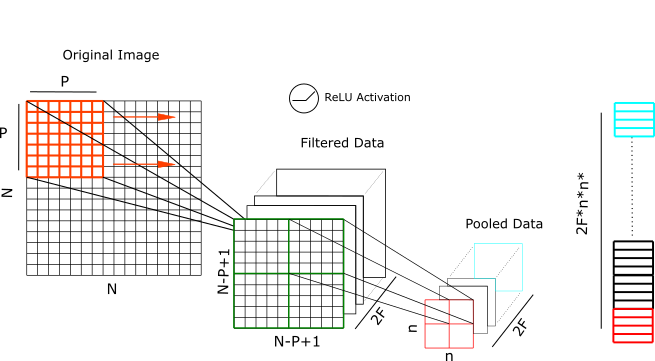
\includegraphics[width = 8cm]{img/CNN.png}
    \caption{\label{fig:cnn}
    An example architecture of a CNN.
    On the left is an 2D image input, followed by a convolutional layers, and a 
    max pooling layer. }
\end{figure}

The convolution layer is defined as a set of filters and an activation function. It convolves the input with the filters and passes the output through the activation function. In the above example, a convolution layer contains $2F$ filters of size $P\times P$. By convolving the $N\times N$ input with all of its filters with a stride length of 1, it generates $2F$ feature maps with size $(N-P+1)\times (N-P+1)$. The stride length defines how many pixels the filters are moved each time. The final output of a convolution layer are obtained by passing the feature maps through the Rectified Linear Unit (ReLU) function defined as
\begin{align}
	\textrm{ReLU}(x) = \max(0,x).
\end{align}

The max-pooling layer scales down the feature maps by dividing them into subsections and representing the entire subsection with its maximum value. At the end of the last max-pool layer, the feature maps are flattened into a vector which are usually used as the input to the fully connected layers shown in Figure \ref{fig:fullyconnected}.

In the fully connected layer (FC), each node has a weighted connection to every node from the previous layer and its output is determined by passing through the weighted sum of its input through an activation function. The flattened feature maps undergo multiple non-linear transformations through several FCs which enables the neural net to find a linear separating plane between classes.\\

\begin{figure}[hb]
	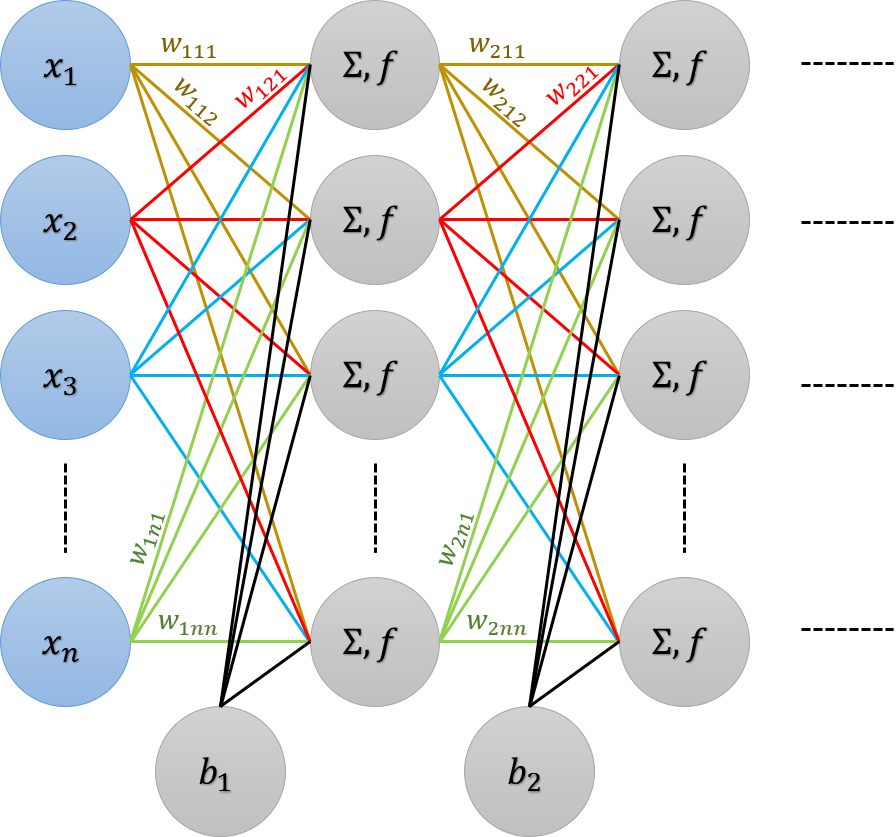
\includegraphics[width = 8cm]{img/fullyconnected.png}
    \caption{\label{fig:fullyconnected}
    Fully connected layers}
\end{figure}

\subsection{All Convolutional Architecture and Model Description}
As the authors observe that top entries in the 2014 Imagenet challenge have architectures that deviated from conventional CNNs, they posed the following problem: which components of CNNs are actually required for achieving state-of-the-art performance. Springennerg et.al began with the simplest architecture of a homogeneous network of only convolutional layers with vanilla stochastic gradient descent with momentum using ReLU as the activation function. This model (All-CNN-C) was able to reach state-of-the-art performance as detailed in Table ~\ref{SFA}.

\begin{table}
  \centering
  \begin{tabular}{|c c c|}
    \hline
    Model & Error (\%) & \# Parameters \\
    \hline
    Model A & 12.47\% & $\approx$ 0.9 M \\
    Strided-CNN-A & 13.46\% & $\approx$ 0.9 M \\
    ConvPool-CNN-A & 10.21\% & $\approx$ 1.28 M \\
    All-CNN-A & 10.30\% & $\approx$ 1.28 M \\
    \hline
    Model B & 10.20\% & $\approx$ 1 M \\
    Strided-CNN-B & 10.98\% & $\approx$ 1 M \\
    ConvPool-CNN-B & 9.33\% & $\approx$ 1.35 M \\
    All-CNN-B & 9.10\% & $\approx$ 1.35 M \\
    \hline
    Model C & 9.74\% & $\approx$ 1.3 M \\
    Strided-CNN-C & 10.19\% & $\approx$ 1.3 M \\
    ConvPool-CNN-C & 9.31\% & $\approx$ 1.4 M \\
    All-CNN-C & 9.08\% & $\approx$ 1.4 M \\
    \hline
  \end{tabular}
  \caption{Original Classification Error on CIFAR-10}
  \label{SFA}
\end{table}

The paper then compares the $p$-norm subsampling (pooling) equation with the standard formulation for defining a convolutional layer. In the pooling equation, $f$ is the feature map produced by some layer of a CNN described as a 3-dimensional array of size $W \times H \times N$. $W$, $H$ and $N$ are the width, height and number of channels respectively. The pooling function $s$ is applied to the feature map $f$ with $k$ as the pool size and $r$ the stride length which gives the following entries: 

\begin{align}
s_{i,j,u}(f) = \bigg ( \sum_{h = - \lfloor k/2 \rfloor}^{\lfloor k/2 \rfloor} \sum_{w = - \lfloor k/2 \rfloor}^{\lfloor k/2 \rfloor} |f_{g_{(h,w,i,j,u)}}|^{p} \bigg ) ^{1/p} 
\end{align}

\noindent where $g_{(h,w,i,j,u)} = (r \dot i + h, r \dot j + w, u)$ is the function mapping the positions in $s$ to $f$ with respect to $r$. As $p \rightarrow \infty$, $s$ becomes max pooling. We know that as long as $r > k$, the pooling regions will not overlap but currently conventional CNNs have $k = 3$ and $r = 2$. 

A convolutional layer applied to a feature map $f$ gives the following entries:

\begin{align}
c_{i,j,o}(f) = \sigma \bigg ( \sum_{h = - \lfloor k/2 \rfloor}^{\lfloor k/2 \rfloor} \sum_{w = - \lfloor k/2 \rfloor}^{\lfloor k/2 \rfloor} \sum_{u=1}^N \theta_{h,w,u,o} \dot |f_{g_{(h,w,i,j,u)}}|\bigg ) 
\end{align}

\noindent where $\theta$ are the convolutional/filter weights, $\sigma(\dot)$ the activation function which in this case is ReLU $\sigma(x) = \max(x, 0)$ and $o \in [1, M]$ being the number of output features of the layer.

When viewed in this form, the similarities between the two equations are strikingly obvious:
\begin{itemize}
\item The ReLU from the convolutional is equivalent to $p \rightarrow \infty$ a.k.a. max
\item Setting $o$ to 3 gives 3 output images (one for each channel) which is the same as having 3 pooled images
\item Having $r$ to be 2 and $k$ to be 3 in the convolutional layer is the same as having a stride of 2 and pool size of 3
\item Both take the feature map as input
\end{itemize}
Hence with $\theta$ set to 1, the convolutional layer is essentially the same as a pooling layer which begs the question whether and why pooling layers are required in the network.

Springenberg et al. gave 3 possible explanations of why pooling helps in CNNs:
\begin{enumerate}
\item The p-norm makes the representation more invariant
\item The spatial dimensionality reduction through pooling enables increasing coverage of the input in higher layers
\item The non-mixing of features in pooling (versus the mixing of features in the convolutional layer through the convolution operation) makes optimization easier
\end{enumerate}

Assuming that only the second reason is why pooling leads in achieving good results, we can replace the max pooling layers with convolutional layers since spatial dimensionality reduction can be lso performed by using a convolutional layers with increased stride; thus pooling layers can be eliminated entirely. The authors then list 2 methods to do so: 1. change the stride of the convolutional layer before the pooling layer to 2 or 2. have a convolutiona layer with filter size 3, stride 2 and output equal to the number of channels.

The set of experiments presented in the paper demonstrated that using convolutional layers with small filter sizes performs better than layers with larger filter sizes. This confirms the results previously obtained by Simonyan and Zisserman \cite{simonyan2014very} where they state that using smaller filter sizes but deeper architectures outperforms larger filter sizes and shallower architectures. An intuitive reason is smaller filter sizes means fewer parameters in a network which prevents overfitting and acts as a mean of regularization.

For example, for an input of size H $\times$ W $\times$ C and one convolutional layer with filter size $7 \times 7$ and stride 1 has $49C$ weights. On the other hand, for the same input and three convolutional layers with filter size $3 \times 3$, stride 1 and padding zeros to preserve the original height and width, has $27C$ weights. In the latter example, a unit in the third layer of the second architecture covers a $7 \times 7$ area of the original input. Therefore, it covers the same area that a unit of the first architecture but with less parameters.

Moreover, the authors also argue that using fully connected layers at the end of the network is not necessary when the architecture is sufficiently deep as the units in the last layer of the network cover an area large enough to recognize the image.

Due to time constraints we were not able to properly implement the devolution approach proposed in the paper. 
